% \RequirePackage{float} % Need to load the float package before hyperref, so hyperref detects and patches it, so when we load minted later it uses the patched \newfloat (minted loads float). More info here: http://tex.stackexchange.com/questions/19371/minteds-listing-environment-with-hyperref-and-caption-package-together

% % Need to do this before
% \makeatletter
% \renewcommand*{\listof}[2]{%
%   \@ifundefined{ext@#1}{\float@error{#1}}{%
%     \expandafter\let\csname l@#1\endcsname \l@figure  % <- use layout of figure
%     \float@listhead{#2}%
%     \begingroup
%       \setlength\parskip{0pt plus 1pt}%               % <- or drop this line completely
%       \@starttoc{\@nameuse{ext@#1}}%
%     \endgroup}}
% \makeatother

% Need to do this before loading hyperref and minted ??
% But can't do this before \documentclass{book} (because it doesn't work then..)
% \RequirePackage{etoolbox}
% \makeatletter
% \patchcmd{\@chapter}%
%  {\addtocontents{lof}}%
%  {\addtocontents{lol}{\protect\addvspace{10pt}}%  % <-- "alg" is the extension you use
%   \addtocontents{lof}}%
%  {\typeout{*** SUCCESS ***}}{\typeout{*** FAIL ***}}
% \makeatother

\documentclass[twoside,english,a4paper]{uiofysmaster}
\usepackage{lmodern}
\usepackage[T1]{fontenc}
\usepackage[utf8]{inputenc}
% \usepackage[top=1.5in, bottom=1.5in, left=1in, right=1in]{geometry} % Correct geometry in uiofysmaster

% ----  biblatex ---- %
\usepackage[english]{babel}
\usepackage{csquotes} % required by {babel} (or biblatex?)
\usepackage[backend=biber, sorting=none, style=numeric]{biblatex} % Note that "sorting=none" is NOT the same as leaving the field blank, "sorting=none" means "sorting=citeorder".
\bibliography{JabRef_database,Mendeley_database}

% ---- Code syntax highlighting ---- %
% \usepackage[scaled=0.8]{beramono}  % Better monospaced font, nice ~ and ^
\usepackage[scale=0.85]{droidmono}

% Order: float - (fix \listoflistings) - hyperref - minted
\usepackage{float}

% Fix listoflistings (need to do this before loading hyperref)
% Fix \listoflistings
\usepackage{etoolbox}
% \newfloat{listing}{h}{lol} % Not necessary
\makeatletter
\patchcmd{\@chapter}%
 {\addtocontents{lof}}%
 {\addtocontents{lol}{\protect\addvspace{10pt}}%  % <-- "lol" is the extension minted use
  \addtocontents{lof}}%
\makeatother

% FIX LIST OF LISTINGS: 
% http://tex.stackexchange.com/a/58498/31078
% http://tex.stackexchange.com/questions/14856/change-spacing-between-elements-in-newfloat-listof/14867#14867
% http://tex.stackexchange.com/questions/139533/using-listing-with-minted-gets-wrong-listoflistings


% Load hyperref after fixing listoflistings
\usepackage{hyperref}
\input{preamble/hyperref.tex}

% Finally load minted
\usepackage[chapter]{minted} % Option [chapter] has to do with \listoflistings numbering. Alternative is ``section''
% Need to load the float package before hyperref, so hyperref detects and patches it, so when we load minted later it uses the patched \newfloat (minted loads float). 
% More info here: http://tex.stackexchange.com/questions/19371/minteds-listing-environment-with-hyperref-and-caption-package-together

\usemintedstyle{colorful}
\definecolor{codebg}{rgb}{0.95,0.95,0.95}
\newminted[cppcode]{mdcpp}{ % can use \newminted{cpp} to replace default ``cpp'', gives the same result
    mathescape,
%     frame=lines,
%     framesep=2mm,
    bgcolor = codebg,
    fontsize = \small,
%     fontfamily = courier
} 
% usage: \begin{cppcode}
% use \begin{cppcode*}{<extra options>} if you want to add extra options on the fly

% More options:
% \renewcommand\listingscaption{Program code}
% \renewcommand\listoflistingscaption{List of program codes}

% FIX LIST OF LISTINGS: 
% http://tex.stackexchange.com/a/58498/31078
% http://tex.stackexchange.com/questions/14856/change-spacing-between-elements-in-newfloat-listof/14867#14867
% http://tex.stackexchange.com/questions/139533/using-listing-with-minted-gets-wrong-listoflistingscaption



% ----  Draft stuff (remove before final version) ---- %
\usepackage{todonotes}
\usepackage{xcolor}
\newcommand{\orangebox}[1]{
    \fcolorbox{black}{orange}{
        \begin{minipage}{\textwidth}
            #1
        \end{minipage}
    }
}
\usepackage{soulutf8}       % To highlight stuff (when using utf8), using \hl{}. Also has \st{} for strikethrough. Doesn't work that well with equations...
\usepackage{lipsum}

% ---- Images ---- %
\usepackage{graphicx}
\usepackage{svg}            % To include .svg vector graphics directly using \includesvg (will automatically compile/convert the images to .pdf+.pdf_tex using Inkscape). 
                            % NEEDS ``pdflatex --shell-escape'' !!!
                            
\setsvg{                    % conversion options for svg package
    inkscape = inkscape -z -D
}

% The subfigure and subfig packages are deprecated and shouldn't be used any more: 
% http://tex.stackexchange.com/questions/144782/subfigure-and-subfig-packages-deprecated
% the svg-package originally uses subfig, but replacing subfig with subcaption seems to work
\usepackage{subcaption}     % \begin{subfigure}, \subcaption{}, and \subcaptionbox{}

% ---- Fix unicode stuff ---- %
\DeclareUnicodeCharacter{2212}{-}   % Unicode 'MINUS SIGN' (U+2212) that matplotlib uses for minus on axis tick labes

% ---- Formatting ---- %
% skip line instead of indent on new paragraph
% \setlength{\parskip}{11pt}
% \setlength{\parindent}{0mm}
\usepackage[parfill]{parskip} % The option parfill is a useful addition: it avoids that a paragraph ends almost flush right. So, paragraphs could easier be distinguished.

% ---- Floats ---- %
% With \renewcommand{\floatpagefraction}{.8}% I was able to specify that only pages with more than 80% of floats, will become pure float-only pages. The default is 0.6 so if a figure consumes 60% of the page it will get its own float-page.
\renewcommand{\floatpagefraction}{.8}

% There are four counters that control how many floats can go into areas:
% totalnumber (default 3) is the maximum number of floats on a text (!) page
% topnumber (default 2) is the maximum number of floats in the top area
% bottomnumber (default 1) is the maximum number of floats in the bottom area
% dbltopnumber (default 2) is the maximum number of full sized floats in two-colum mode going above the text columns.
\setcounter{totalnumber}{6}
\setcounter{topnumber}{4}
\setcounter{bottomnumber}{2}

%TODO:
% Consider increasing +- ranges?
% Show defaults using \showthe\textfloatsep or \the\textfloatsep
% See here for defaults: http://tex.stackexchange.com/a/23316/31078
% See image here for illustration of space: http://tex.stackexchange.com/a/60479/31078
% Defaults for uiofysmaster using default font size
% \floatsep:        12.0pt plus 2.0pt minus 4.0pt
% \textfloatsep:    20.0pt plus 2.0pt minus 4.0pt
% \intextsep:       14.0pt plus 4.0pt minus 4.0pt
% \dbltextfloatsep: 20.0pt plus 2.0pt minus 4.0pt
% \dblfloatsep:     14.0pt plus 2.0pt minus 4.0pt
\setlength{\textfloatsep}{8.0pt plus 6.0pt minus 2.0pt} % 20.0pt plus 2.0pt minus 4.0pt
\setlength{\intextsep}{8.0pt plus 6.0pt minus 2.0pt} % 14.0pt plus 4.0pt minus 4.0pt 
\setlength{\floatsep}{8.0pt plus 4.0pt minus 2.0pt} % 12.0pt plus 2.0pt minus 4.0pt

% ---- Captions ---- %
% \usepackage{caption} % Loaded by uiofysmaster
\captionsetup[table]{width=.9\textwidth,position=above}
\captionsetup[figure]{width=.9\textwidth,position=below}
\captionsetup[listing]{width=.9\textwidth,position=below}
% \captionsetup{font=small,labelfont=bf} % In uiofysmaster
\captionsetup[subfigure]{position=below}

% See image here for illustration of space: http://tex.stackexchange.com/a/60479/31078
% See here for defaults: http://tex.stackexchange.com/a/23316/31078
% Show defaults using \showthe\textfloatsep or \the\textfloatsep
% Defaults for uiofysmaster using default font size
% \abovecaptionskip: 10.0pt
% \belowcaptionskip:  0.0pt
\setlength{\belowcaptionskip}{0.0pt} % 0.0pt
\setlength{\abovecaptionskip}{8.0pt} % 10.0pt


% ---- Other stuff ---- %
% \usepackage{minipage}
\usepackage{commath}        % To correctly typeset differentials \od[2]{f}{x}, \dod, and \tod
\usepackage{fancyvrb}       % Better verbatim, that works inside fcolorbox. Usage: \begin{Verbatim} or \Verb!verbatimThing!
\usepackage{cleveref}       % Use \cref{fig:label} instead of \ref{} to get auto ``fig. 1.1a''. \Cref for capitalized.
\usepackage{upgreek}        % Upper case greek letters
\usepackage{bm}             % Bold symbols in math mode
\usepackage{mathtools}      % Mainly for \vdotswithin{=} and \shortvdotswithin{=}
\usepackage{pdfpages}       % To include the frontpage pdf
% \usepackage{hyperref}       % Load hyperref package last % Loaded by uiofysmaster
% \usepackage{paralist}
\usepackage{relsize}        % To resize stuff - specifically integration signs
\usepackage{exscale}        % To resize integration sign twice, ``\DeclareMathOperator{\biggerint}{\mathlarger{\mathlarger{\int}}}''
\usepackage{braket}         % Dirac bra/kets, \Bra{a}, \Ket{b}, \Braket{a|b|a}. \Braket auto stretches \l/rangles and |'s
% \usepackage{float}        % Put at top of master using \RequirePackage{float}, to fix minted/hyperref/float
\usepackage{placeins}       % Stop floats from going past somewhere by adding \FloatBarrier. This makes all floats before the barrier appear before the barrier in the pdf

% ---- Custom itemize ---- %
\usepackage{enumitem}       % Better control over enu­mer­ate, item­ize and de­scrip­tion. Su­per­sedes both enu­mer­ate and md­wlist.
\SetEnumitemKey{midsep}{topsep=3pt,partopsep=3pt,parsep=3pt,itemsep=3pt}

% ---- Custom lengths for figures ---- %
% (so we can just use \setlength later)
\newlength{\myfigwidth}
\newlength{\mycaptionwidth}

% ---- Custom commands and symbols ---- %
% ----- Vectors ---- %
% \newcommand{\bvec}[1]{\mathbf{#1}}
\newcommand{\bvec}[1]{\boldsymbol{#1}}    % Using amsmath's boldsymbol
% \newcommand{\bvec}[1]{\bm{#1}}
\newcommand{\rvec}{\bvec{r}}
\newcommand{\vvec}{\bvec{v}}
\newcommand{\avec}{\bvec{a}}
\newcommand{\Fvec}{\bvec{F}}
% ---- Other math commands and symbols ---- %
% \newcommand\diff{\mathop{}\!\mathrm{d}}   % Already defined as \dif by commath! But maybe this way is better? Commath uses ``\DeclareMathOperator{\dif}{d \!}''
\DeclareMathOperator{\diff}{d \!}           % See top comment on this reply: http://tex.stackexchange.com/a/95681/31078
% \newcommand\Ham{\mathop{}\!\mathrm{\mathcal{H}}}
\DeclareMathOperator{\Ham}{\mathcal{H}}
% \newcommand\bigint{\mathop{\mathlarger{\int}}}
\DeclareMathOperator{\bigint}{\mathlarger{\int}}
% \newcommand\deltaop{\mathop{\!\mathrm{\delta}}}
% \DeclareMathOperator{\deltaop}{\updelta \!}
\DeclareMathOperator{\deltaop}{\updelta}
% \newcommand\biggerint{\mathop{\mathlarger{\mathlarger{\int}}}}
\DeclareMathOperator{\biggerint}{\mathlarger{\mathlarger{\int}}}
% ---- Other ---- %
\newcommand{\Ang}{\AA ngstr\"om}
\newcommand{\Schr}{Schr\"odinger}

% ---- Fix unicode stuff ---- %
\DeclareUnicodeCharacter{2212}{-}   % Unicode 'MINUS SIGN' (U+2212) that matplotlib uses for minus on axis tick labes

% ---- Formatting ---- %
% skip line instead of indent on new paragraph
\setlength{\parskip}{11pt}
\setlength{\parindent}{0mm}
% make figure text more narrow than textwidth, use small font, and make ``figure'' bold
% ! see alternatives in FYS4180 report
\captionsetup{width=.9\textwidth}
\captionsetup{font=small,labelfont=bf}

% % \usepackage{float}
% \makeatletter
% \renewcommand*{\listof}[2]{%
%   \@ifundefined{ext@#1}{\float@error{#1}}{%
%     \expandafter\let\csname l@#1\endcsname \l@figure  % <- use layout of figure
%     \float@listhead{#2}%
%     \begingroup
%       \setlength\parskip{0pt plus 1pt}%               % <- or drop this line completely
%       \@starttoc{\@nameuse{ext@#1}}%
%     \endgroup}}
% \makeatother


\author{Filip Sund}
\title{\uppercase{Water confined in nanoporous media}}
\date{June 2014}

% TODO:
% Decide on caption skips (see preamble)

% \includeonly{molecular_dynamics/simulations}
% \includeonly{fractures/fractures}
\begin{document}

\pagenumbering{roman}
\includepdf{frontpage.pdf}
\cleardoublepage

\begin{abstract}
\todoa{Check distance before and after \AA and \cpp and similar commands}
    \lipsum[1-4]
\end{abstract}
\begin{dedication}
  To someone
  \\\vspace{12pt}
  \lipsum
\end{dedication}
\begin{acknowledgements}
``This work was performed on the Abel Cluster, owned by the University of Oslo and the Norwegian metacenter for High Performance Computing (NOTUR), and operated by the Department for Research Computing at USIT, the University of Oslo IT-department. \url{http://www.hpc.uio.no/}''

Thanks to Ovito\cite{stukowski2010ovito} and Inkscape\cite{webinkscape}

\end{acknowledgements}


\tableofcontents

\listoffigures
\listoftables
\listoflistings

\chapter*{Introduction}%
\addcontentsline{toc}{chapter}{Introduction}%
In this chapter we will give an overview of how simulations of atomic systems are done using molecular dynamics. We will show the theory that makes molecular dynamics so efficient and powerful, and we will show how to build up and implement a molecular dynamics program. 

The program used for producing the results presented later in this thesis uses a much more sophisticated model for the interactions between the atoms than is presented in this chapter, and is parallellized and highly optimized for doing calculations on high-performance computing clusters like Abel. We will nevertheless gain a lot of insight into this program by starting with a a simpler case.

% To accurately study molecular many-body systems like water confined in nanoporous silica means that we have to consider the quantum mechanical nature of atoms and molecules. To study the motion of atoms using \hl{ab-initio} quantum mechanical calculations, where we have to consider the effect of all electrons, protons and neutrons for all atoms, we have to solve a problem with dimensionality 
% 
% To study water confined in nanoporous silica we use the the method of molecular dynamics simulations. This is a method that use knowledge from the complex quantum mechanical nature of atoms and molecules, to reduce the many-body problems  create simple potentials only depending on the positions \hl{(and velocities?)} of atoms represented as point particles, which we can integrate using Newton's equations of motion. 
% 
% to replacing heavy calculations on the wavefunctions of electrons, protons and neutrons with simple\hl{r} calculations only depending on the positions \hl{(and velocities?)} of point particles representing the positions of the atoms.
% 
% where we approximate the forces between atoms using potentials and parameters from studies and simulations of the underlying quantum mechanical nature of the atoms. This means that we don't have to calculate the exact quantum mechanical interactions between atoms, but instead model the atoms as point particles, with potentials depending on the positions \hl{(and velocities)} of the atoms that give rise to forces. By integrating the forces using Newton's equations of motion
% 
% To do an exact study of the behaviour of atoms and molecules we have to take into account the quantum mechanical workings of such a system. To a silica system we have to consider the that silicon and oxygen consist of  electrons, protons and neutrons of all atoms 

We want to study water confined in nanoporous silica. We choose to do this on an atomic scale, using molecular dynamics. Studies of similar studies have been performed using the same methods, so we expect this method will produce good results. A different approach could be a statistical study, using something like Direct Simulation Monte Carlo (DSMC).

To do an exact study of a many-body atomic system like water confined in nanoporous silica, we have to take into account the quantum mechanical nature of the atoms and molecules in the system. An oxygen molecule consists of 8 electrons, 8 protons and 8 neutrons, all interacting with each other, and each with 3 translational degrees of freedom. This makes doing calculations on something that might appear simple, pretty complex if we want to do it properly. If we want to study a system consisting of more than a couple of oxygen atoms we see that the number of particles and degrees of freedom quickly makes the problem grow to intractable proportions. Since we are mainly interested in the equilibrium and transport properties of the system, we can reduce the problem to something we can handle by using results from underlying quantum mechanical calculations, and experimental studies, to develop approximate models of the system. We do this by assuming that the many-body system behaves clasically, and model all atoms as point particles. We further create potentials from quantum mechanical results that approximate the exact forces between the atoms, and adjust the parameters of these potentials to fit experimental and computational results. These potentials only depend on the positions of the atoms we want to simulate, which is orders of magnitude faster to evaluate than calculating the exact forces between the atoms from quantum mechanical principles. We then solve Newton's equations of motion for the system to evolve the system in time.

% To explain how a Molecular Dynamics simulation work we start with a simple example, using one atom type, and a simple model for the force between the atoms. This allows us to get an understanding of the basic concepts used in \hl{MD}. The program actually used for the calculations in the work presented in this thesis uses a very complex potential, and is highly optimized and parallellized for doing calculations on computing clusters on several hundred \hl{CPU's}. But the inner workings of that program \hl{is both a) too much to cover? and b) not necessary to explain?).}

After presenting a simple molecular dynamics model we briefly mention some methods for optimizing such a program, before we look at what we are able to study using a molecular dynamics simulation. We first look at how to measure the temperature and pressure in a system, before we look at how to study different ensembles using so-called \emph{thermostats}, which can control the temperature, pressure, or other physical proterties of a system. We conclude this chapter with an overview of the program used for producing the results presented later in this thesis, which we use to model silicon dioxide (silica), and water trapped inside nanoporous silica.

\part{Molecular dynamics}
    \chapter*{Introduction}%
\addcontentsline{toc}{chapter}{Introduction}%
In this chapter we will give an overview of how simulations of atomic systems are done using molecular dynamics. We will show the theory that makes molecular dynamics so efficient and powerful, and we will show how to build up and implement a molecular dynamics program. 

The program used for producing the results presented later in this thesis uses a much more sophisticated model for the interactions between the atoms than is presented in this chapter, and is parallellized and highly optimized for doing calculations on high-performance computing clusters like Abel. We will nevertheless gain a lot of insight into this program by starting with a a simpler case.

% To accurately study molecular many-body systems like water confined in nanoporous silica means that we have to consider the quantum mechanical nature of atoms and molecules. To study the motion of atoms using \hl{ab-initio} quantum mechanical calculations, where we have to consider the effect of all electrons, protons and neutrons for all atoms, we have to solve a problem with dimensionality 
% 
% To study water confined in nanoporous silica we use the the method of molecular dynamics simulations. This is a method that use knowledge from the complex quantum mechanical nature of atoms and molecules, to reduce the many-body problems  create simple potentials only depending on the positions \hl{(and velocities?)} of atoms represented as point particles, which we can integrate using Newton's equations of motion. 
% 
% to replacing heavy calculations on the wavefunctions of electrons, protons and neutrons with simple\hl{r} calculations only depending on the positions \hl{(and velocities?)} of point particles representing the positions of the atoms.
% 
% where we approximate the forces between atoms using potentials and parameters from studies and simulations of the underlying quantum mechanical nature of the atoms. This means that we don't have to calculate the exact quantum mechanical interactions between atoms, but instead model the atoms as point particles, with potentials depending on the positions \hl{(and velocities)} of the atoms that give rise to forces. By integrating the forces using Newton's equations of motion
% 
% To do an exact study of the behaviour of atoms and molecules we have to take into account the quantum mechanical workings of such a system. To a silica system we have to consider the that silicon and oxygen consist of  electrons, protons and neutrons of all atoms 

We want to study water confined in nanoporous silica. We choose to do this on an atomic scale, using molecular dynamics. Studies of similar studies have been performed using the same methods, so we expect this method will produce good results. A different approach could be a statistical study, using something like Direct Simulation Monte Carlo (DSMC).

To do an exact study of a many-body atomic system like water confined in nanoporous silica, we have to take into account the quantum mechanical nature of the atoms and molecules in the system. An oxygen molecule consists of 8 electrons, 8 protons and 8 neutrons, all interacting with each other, and each with 3 translational degrees of freedom. This makes doing calculations on something that might appear simple, pretty complex if we want to do it properly. If we want to study a system consisting of more than a couple of oxygen atoms we see that the number of particles and degrees of freedom quickly makes the problem grow to intractable proportions. Since we are mainly interested in the equilibrium and transport properties of the system, we can reduce the problem to something we can handle by using results from underlying quantum mechanical calculations, and experimental studies, to develop approximate models of the system. We do this by assuming that the many-body system behaves clasically, and model all atoms as point particles. We further create potentials from quantum mechanical results that approximate the exact forces between the atoms, and adjust the parameters of these potentials to fit experimental and computational results. These potentials only depend on the positions of the atoms we want to simulate, which is orders of magnitude faster to evaluate than calculating the exact forces between the atoms from quantum mechanical principles. We then solve Newton's equations of motion for the system to evolve the system in time.

% To explain how a Molecular Dynamics simulation work we start with a simple example, using one atom type, and a simple model for the force between the atoms. This allows us to get an understanding of the basic concepts used in \hl{MD}. The program actually used for the calculations in the work presented in this thesis uses a very complex potential, and is highly optimized and parallellized for doing calculations on computing clusters on several hundred \hl{CPU's}. But the inner workings of that program \hl{is both a) too much to cover? and b) not necessary to explain?).}

After presenting a simple molecular dynamics model we briefly mention some methods for optimizing such a program, before we look at what we are able to study using a molecular dynamics simulation. We first look at how to measure the temperature and pressure in a system, before we look at how to study different ensembles using so-called \emph{thermostats}, which can control the temperature, pressure, or other physical proterties of a system. We conclude this chapter with an overview of the program used for producing the results presented later in this thesis, which we use to model silicon dioxide (silica), and water trapped inside nanoporous silica.
    \chapter{Statistical mechanics}
% \hl{The idea behind Molecular Dynamics simulations is that we can study the average behaviour of a many-body system by computing the natural time evolution of the system numerically and averaging the quantity of interest over a sufficiently long time.} -- Frenkel p. 15
% 
% Before we start work on to do simulations using molecular dynamics, we need some basics on \emph{why} we can use MD to study atomic systems like silica and water. We first use the Born-Oppenheimer approximation to justify that the Hamiltonian of the system can be expressed as a function of the positions and velocities of the atoms, having averaged out the rapid motion of the individual subatomic particles (like electrons and protons). We then make the approximation that a classical description of the system is adequate, which we 
% 
% % To do this we need some \hl{something} from the field of statistical mechanics.
% 
% Using statistical mechanics stated in quantum mechanical terms, and using
% 
% The basic assumption behind statistical mechanics, from which much of statistical mechanics follows, is that a system with fixed number of particles $N$, volume $V$ and energy $E$ is equally likely to be found in any of its eigenstates. Using this assumption, and stating statistical mechanics in quantum mechanical terms, it can be shown that the probability for finding a system at temperature $T$ in quantum state $i$ is
% \begin{align}
% %     P_i = 
%     \frac{\exp\left(-\beta E_i\right)}{\sum_j \exp\left( -\beta E_j\right)},
%     \label{eq:boltzmann}
% \end{align}
% where $\beta = 1/k_B T$, $k_B$ is the Boltzmann constant, $E_i$ is the energy of a system in state $i$, and the sum in the divisor goes over all states at temperature $T$. This equation is the well-known Boltzmann distribution for a system at temperature $T$. From \cref{eq:boltzmann} it can be shown that the thermal average of an observable $A$ can be computed as
% \begin{align}
%     \langle A \rangle =
%     \frac{
%         \sum_i \exp \left( -\beta E_i \right) \Braket{i|A|i}
%     }{
%         \exp \left( -\beta E_i \right)
%     },
%     \label{eq:quantum_thermal_average}
% \end{align}
% where $\Braket{i|A|i}$ is the expectation value of the operator $A$ in quantum state $i$. The problem is that to compute a thermal average like this, we have to solve the \Schr~ equation for an arbitray many-body system, which is, in general, an untractable problem. Even if we could, the number of quantum states that contribute to the average in \cref{eq:quantum_thermal_average} would be so astronomically large ($\mathcal{O}(10^{10^{25}})$) that a numerical evaluation of all expectation values would be impossible.
% 
% Fortunately \cref{eq:quantum_thermal_average} can be simplified in the classical limit, where we consider \hl{actions} on a scale much larger than $\hbar$, meaning that we can ignore\todo{somethings}. In the classical limit we get
% \begin{align*}
%     \left\langle A\right\rangle = \frac
%     {
%         \bigint \dif \bvec r^N \dif \bvec p^N \exp 
%         \left\{
%             -\beta \Ham \left( \bvec r^N, \bvec p^N \right)
%         \right\} 
%         A\left(\bvec r^N, \bvec p^N\right)
%     }
%     {
%         \bigint \dif \bvec r^N \dif \bvec p^N \exp 
%         \left\{
%             -\beta \Ham\left( \bvec r^N, \bvec p^N \right)
%         \right\}
%     },
% \end{align*}
% where $\Ham$ is the Hamilton operator
% \begin{align*}
%     \Ham(\bvec r^N, \bvec p^N) = 
%         U(\rvec^N) + \sum_i^N \frac{p_i^2}{2m_i},
% \end{align*}
% $\bvec r^N$ is the position of all the atoms, $\bvec p^N$ is the corresponding momenta, $m_i$ is the mass of atom $i$, and $U$ is the potential energy of the system.
% 
% So far we have seen that the 
% 
% average value of an observable $A$ can be computed as
% \begin{align*}
%     \langle A \rangle =
%     \frac{
%         \sum_i \exp \left( -\beta E_i \right) \Braket{i|A|i}
%     }{
%         \exp \left( -\beta E_i \right)
%     },
% \end{align*}
% where $i$ denotes the quantum state of a system, the sum $\sum_i$ goes over all  $\beta = 1/k_B T$, $k_B$ is the Boltzmann constant, $T$ is the temperature, $E_i$ is the energy of a system 
% 
% 
% time average of a physical quantity
% \begin{align*}
%     \bar A = \lim_{T\rightarrow \infty} \frac{1}{T} \int_0^T A(t) \dif t
% \end{align*}
% then using classical mechanics, classical limit, NVE ensemble
% denoting the state of the system as $X$, and the sum over all states with a fixed energy $E$ as $\sum_{\{X|E\}}$
% \begin{align*}
%     \langle A \rangle = 
%     \frac{
% %         \displaystyle
%         \sum_{\{X|E\}} A(X)
%     }{
% %         \displaystyle
%         \sum_{\{X|E\}}
%     }
%     =
%     \frac{
% %         \displaystyle
%         \sum_X A(X) \deltaop \left[ \Ham(X) - E \right]
%     }{
% %         \displaystyle
%         \sum_X \deltaop \left[ \Ham(X) - E \right]
%     }
%     = \bar A
% \end{align*}
% in the sums on the right had side the delta-function $\deltaop[\Ham(X)-E]$ restricts the sum to states with energy $E$
% 
% 
% in the classical limit we can write the \hl{thermal???} average of an observable $A$ as\cite{frenkel2001understanding}\todo{eq. (2.2.6), p. 13 + eq. (3.1.2) p. 23}
% % \begin{align*}
% %     \left\langle A\right\rangle = \frac
% %     {
% %         \biggerint \dif \bvec p^N \dif \rvec^N \exp \left\{ -\beta
% %             \left[ 
% %                 \sum_i \frac{p_i^2}{2m_i} + U(\rvec^N)
% %             \right]
% %         \right\} 
% %         A(\bvec p^N, \bvec q^N)
% %     }
% %     {
% %         \biggerint \dif \bvec p^N \dif \rvec^N \exp \left\{ -\beta
% %             \left[ 
% %                 \sum_i \frac{p_i^2}{2m_i} + U(\rvec^N)
% %             \right]
% %         \right\}
% %     }
% % \end{align*}
% \begin{align*}
%     \left\langle A\right\rangle = \frac
%     {
%         \bigint \dif \bvec r^N \dif \bvec p^N \exp 
%         \left\{
%             -\beta \Ham \left( \bvec r^N, \bvec r^N \right)
%         \right\} 
%         A\left(\bvec r^N, \bvec p^N\right)
%     }
%     {
%         \bigint \dif \bvec r^N \dif \bvec p^N \exp 
%         \left\{
%             -\beta \Ham\left( \bvec r^N, \bvec r^N \right)
%         \right\}
%     },
% \end{align*}
% where $\beta = 1/k_B T$, $T$ is the temperature, $k_B$ is the Boltzmann constant, $\bvec r^N$ is the positions of all $N$ atoms, and $\bvec p^N$ the corresponding momenta. The function $\Ham(\bvec r^N, \bvec p^N)$ is the Hamiltonian of the system, and can be expressed as
% \begin{align*}
%     \Ham(\bvec r^N, \bvec p^N) = 
%         U(\rvec^N) + \sum_i^N \frac{p_i^2}{2m_i}
% \end{align*}
% 
% From this we can show that we can measure for example the average pressure and temperature of a system from the time evolution of those quantities
% \begin{align*}
%     \left\langle \frac{1}{2}mv^2 \right\rangle = \frac{1}{2}k_B T
% \end{align*}
% 
% \todo[inline]{The alternative is Monte Carlo simulations?}



In molecular dynamics we study systems of many interacting atoms and molecules by assuming that they behave classically, and solve Newton's equations of motion using an appropriate integration scheme to evolve the system in time. By assuming that the atoms behave classically we mean that we model the atoms as point particles, and characterize them using their position, $\bvec r$, velocity, $\bvec v$ and the force acting on them, $\bvec f$. The interactions between the atoms, that stem from the quantum mechanical \hl{something}, are described using potentials. It is into these potentials we bake the physical insight of the systems we want to simulate, which we often do by finding potentials using studies and simulations of the underlying quantum mechanical nature of the interactions between the atoms in the system.

    \chapter{A simple molecular dynamics program?}
Intro

\section{The main program}
% Deducing how a molecular dynamics program does its simulations isn't always easy from looking at source code, but most programs will follow a flow similar to the following:
Most molecular dynamics programs will follow an flow similar to the following:
\begin{itemize}[midsep]
    \renewcommand{\labelitemii}{$\bullet$} % Set list depth 2 bullet thing equal to first
    \item Initialize the system. Set up the initial positions and velocities for all atoms, either by generating them or loading a saved state from a previous simulation.\todo{remove drift!}
    \item For each timestep
    \begin{itemize}[midsep]
        \item Calculate the forces between the atoms.
        \item Integrate Newton's equations of motion using an appropriate integration scheme \todo{examples?}.
        \item Sample the values of the quantities we want to study, and add to the averages.
    \end{itemize}
    \item After all timesteps have been finished we print out the measured quantities, and we could also save the state of the system so we can continue from this state later.
\end{itemize}
An example of a program that implements the above procedure can be seen in \cref{list:simple_md_program}.
\begin{listing}[!ht]
\begin{cppcode*}{gobble=4}
    System system = initializeSystem(parameters);
    double time = 0.0;
    double dt = 0.01;
    for (double time = 0; time < tMax; time += dt)
    {
        calculateForces(system);
        integrateEquationsOfMotion(system, dt);
        sample(system);
    }
\end{cppcode*}
\caption{
    An example of a typical implementation of a molecular dynamics program using object-oriented programming.
    \label{list:simple_md_program}
}
\end{listing}

When starting a new simulation we usually initialize the positions of the atoms by putting them on a regular grid like a face-centered cubic (fcc), a body-centered cubic (bcc), or a simple cubic grid. The purpose of this is to not have any atoms too close to each other, which we see from the $r^{-12}$ term would give very big forces\todo{not defined yet... move this section?}, and to start with the atoms in a state from which we are able to quickly get to the state we want to study. If we for example want to study a liquid argon system, it is wise to start in an unstable crystal state, by for example using a low density or high temperature, so that the system would melt spontaneously when we start the simulation.

\section{Calculation of forces}
The forces are calculated from the derivatives of interatomic potentials, that depend on the positions of the atoms, and generally are of the form
\begin{align*}
    U(\rvec) = \sum_{i<j} U_{ij}(r_{ij}) + \sum_{i<j<k} U_{ijk}(\rvec_i, \rvec_i, \rvec_k) + \dots,
\end{align*}
where $\rvec_i$ is the position of atom $i$, $r_{ij}$ is the distance between atom $i$ and $j$, $U_{ij}$ is a two-particle potential depending only on the distance between two atoms, and $U_{ijk}$ is a three-particle potential that usually also depends on the angle between three atoms. Higher-order contributions are also often used\todo{ReaxFF}, but they are very demanding to evaluate numerically.

When developing potentials from quantum mechanical calculations one has to weigh the benefits of having a complex potential that models the interactions accurately, against having a less comples potential that will be easier to implement, and faster to evaluate. The limiting factor in any molecular dynamics calculation is the cost of doing simulations on high-performance computing clusters\hl{like abel}, but luckily it seems like the progress in \hl{CPU} development still seems to follow Moore's Law\hl{source?}, that states that the number of transistors on integrated circuits double approximately every two years\cite{moore1965cramming}, effectively halving the price of doing a computation\hl{source?}.

In this example we will be using a potential first seen as early as 1924\cite{jones1924potential} called the Lennard-Jones potential, \hl{after its creator}. The potential is a simple two-particle potential with the following form
% To model a simple mono-atomic system we use the well-known Lennard-Jones potential\cite{jones1924potential}, which when applied on the noble gas \hl{(inert)} Argon gives results that are in good agreement with experimental results. The potential is usually written as follows
\begin{align}
%     U(r) = 4\varepsilon \Big[
%     \underbrace{
%         \left(\frac{\sigma}{r}\right)^{12}
%     }_{\text{attraction}}
%      - 
%     \underbrace{
%         \left(\frac{\sigma}{r}\right)^6
%     }_{\text{repulsion}}
%     \Big],
    U(r_{ij}) = 4\varepsilon\left[ \left(\frac{\sigma}{r}\right)^{12} - \left(\frac{\sigma}{r}\right)^{6} \right]
    = \varepsilon\left[ \left(\frac{r_m}{r}\right)^{12} - 2\left(\frac{r_m}{r}\right)^{6} \right],
    \label{eq:lennard-jones_potential}
\end{align}
where $\sigma$ is the distance between where the potential is zero \hl{(the equilibrium distance between the atoms)}, $\varepsilon$ is related to the strength of the potential (the minimum value of the potential), and $r_m = 2^{1/6} \sigma$ is the distance where the potential is at its minimum. The $r^{-12}$ term is a repulsive term that describes \hl{Pauli repulsion/steric repulsion/overlap of electron orbitals} and the $r^{6}$ term is an attractive term that describes \hl{long range/van der Waals/dipole-dipole/dispersion} interactions. \todo{something about physical justification, use 6 for repulsive because $r^{12} = (r^6)^2$}. 

The potential was used by Lennard-Jones to study the \hl{noble gas} Argon, and has been used by many others\todo{to study what? Examples}. See \cref{fig:lennard-jones_potential} for a plot of the potential using the parameters usually used for simulating Argon\cite{frenkel2001understanding}, $\sigma = 3.405$~\AA\ and $\varepsilon = 0.010318$~eV.
\begin{figure}[!ht]
    \centering
    \includesvg[width=0.7\textwidth, svgpath=./images/lennard-jones/]{lennard-jones_manualalign}
%     \includesvg[width=0.7\textwidth, svgpath=./images/lennard-jones/]{lennard-jones}
    \caption{
        Plot of the Lennard-Jones potential, as stated in \cref{eq:lennard-jones_potential}. Using the parameters usually used for simulating Argon\cite{frenkel2001understanding}, $\sigma = 3.405$~\AA\ and $\varepsilon = 0.010318$~eV.
        \label{fig:lennard-jones_potential}
    }
\end{figure}

\subsection{Newton's third law}
When calculating two-particle forces like the Lennard-Jones potential there is a simple optimization that lets us halve the number of computations, by utilizing Newton's third law. We see that when evaluating $U(r_{ij})$, the force will have the same magnitude if we switch particle $i$ and $j$. This means that when we have calculated the force $\vec F_{ij}$, from particle $j$ on particle $i$, we know that the force on atom $j$ from particle $i$ will have the same magnitude, and we can simply add the opposite force to atom $j$, $\vec F_{ji} = -\vec F_{ij}$. This way we only have to calculate the forces between particle $i$ and particles $j>i$ in the main force loop.

See \cref{list:calculate_forces,list:calculate_force_between_atoms} for an example of how to implement force calculation using the Lennard-Jones potential, using the optimization from Newton's third law.
\begin{listing}[!ht]
% \begin{cppcode*}{gobble=4}
%     void calculateForces(System &system)
%     {
%         for (Atom *atom1 : system.atoms())
%         {
%             for (Atom *atom2 : system.atoms())
%             {
%                 
%             }
%         }
%     }
% \end{cppcode*}
%         for (vector<Atom*>::iterator atom1 = atoms.begin(); atom1 != atoms.end(); ++atom1)
\begin{cppcode*}{gobble=4}
    void calculateForces(System &system)
    {
        const vector<Atom*> &atoms = system.atoms();
        for (auto atom1 = atoms.begin(); atom1 != atoms.end(); ++atom1)
        {
            // Use Newton's third law to skip half the force calculations
            for (auto atom2 = atom1.next(); atom2 != atoms.end(); ++atom2)
            {
                calculateForceBetweenTwoAtoms(*atom1, *atom2);
            }
        }
    }
\end{cppcode*}
\caption{
%     An example of how to implement the velocity Verlet integration scheme using \cpp-like object-oriented programming.
    Caption.
    \label{list:calculate_forces}
}
\end{listing}
\begin{listing}[!ht]
\begin{cppcode*}{gobble=4}
    vec3 calculateForceBetweenTwoAtoms(Atom *atom1, Atom *atom2)
    {
        vec3 drVec = atom1->position() - atom2->position();
        
        double dr2 = drVec.lengthSquared();
        double dr6 = dr2*dr2*dr2;

        double LJforce = 24.0*(2.0 - dr6)/(dr6*dr6*dr2);
        vec3 force = drVec*LJforce;
        
        atom1->force() += force;
        atom2->force() -= force; // Newton's third law
        
        return force;
    }
\end{cppcode*}
\caption{
%     An example of how to implement the velocity Verlet integration scheme using \cpp-like object-oriented programming.
    Caption.
    \label{list:calculate_force_between_atoms}
}
\end{listing}

\section{Integration scheme}
To integrate the Newton's equations of motion for the intermolecular potential there are a lot of different methods to choose between, ranging from the simple forward Euler method\hl{cite} first described by Leonard Euler in 1768, to higher order predictor-corrector methods\hl{cite}. 

It turns out that a deceptively simple method first described by Loup Verlet in 1967\cite{verlet1967computer} often satisfies our needs in an integrator, being both very accurate over long simulation times, having a \hl{global/accumulated} error of the order $\mathcal{O}(\Delta t^2)$\todo{either \cite{thijssen1999computational} sec. 8.4.1-8.4.3 or \cite{frenkel2001understanding} sec. 4.3.3, or derive self in appendix}., and numerically cheap \hl{(compared to other methods)} \hl{requiring on the order of $N$?? flops}. The Verlet method has many variations, but the simplest form \hl{(the one used/described by Verlet)} has the form
\begin{align}
    \rvec(t + \Delta t) \approx 2\rvec(t) - \rvec(t - \Delta t) + \avec(t)\Delta t^2,
    \label{eq:regular_verlet}
\end{align}
where $\Delta t$ is the timestep\todo{define timestep}, and $\avec(t)$ is the velocity at time $t$. This form of the scheme has a truncation error in the position for one timestep of the order $\mathcal{O}(\Delta t^4)$ \hl{show this}.

The stability and \hl{versatiliy} of the \hl{velocity} Verlet method comes from the fact that the scheme is symplectic\todo{show this?, appendix material}. \hl{write more about this, what this means}.

We see that the velocity isn't explicitly calculated or used in this form of the sceme, but if we need it for our experiments we can estimate the velocity using a Taylor expansion around $\rvec(t\pm\Delta t)$, which gives
\begin{align*}
    \vvec(t) = \frac{\rvec(t + \Delta t) - \rvec(t - \Delta t)}{2\Delta t},
\end{align*}
which has a truncation error for one timestep of the order $\mathcal{O}(\Delta t^2)$ \hl{show this}. 

The implementation of the Verlet scheme is mostly straightforward, the only thing we have to take care of happens in the first step. When calculating the positions in the first step, $\rvec(0+\Delta t)$, we see from \cref{eq:regular_verlet} that we need the positions from the previous step, $\rvec(0-\Delta t)$. These positions are usually \hl{simply} approximated using the initial velocity, as follows\todo{is this bad?}
\begin{align*}
    \rvec(0-\Delta t) = \rvec(0) - \vvec(0)\Delta t.
\end{align*}
See \cref{list:regular_verlet} for an example of how to implement the Verlet integration scheme.

\begin{listing}[!ht]
\begin{cppcode*}{gobble=4}
    void integrateEquationsOfMotion(System &system, double dt)
    {
        for (Atom *atom : system.atoms())
        {
            vec3 newPosition = 2.0*atom->position() - atom->oldPosition() 
                               + atom->force()*dt*dt;
            atom->oldPosition() = atom->position();
            atom->position() = newPosition;
            atom->velocity() = (atom->position() - atom->oldPosition())
                               /(2.0*dt);
        }
    }
\end{cppcode*}
\caption{
%     An example of how to implement the velocity Verlet integration scheme using \cpp-like object-oriented programming.
    Caption.
    \label{list:regular_verlet}
}
\end{listing}

The most used form of the Velocity integration scheme is called the velocity Verlet method\cite{swope1982computer}, and it has the form
\begin{align}
    \rvec(t + \Delta t) &= \rvec(t) + \vvec(t)\Delta t + \avec(t)\frac{\Delta t^2}{2}, \label{eq:velocity_verlet_position}\\
    \vvec(t + \Delta t) &= \vvec(t) + \big[\avec(t) + \avec(t + \Delta t)\big] \frac{\Delta t}{2}, \label{eq:velocity_verlet_velocity}
\end{align}
with the truncation error for one timestep $\Delta t$ being of the order $\mathcal{O}(\Delta t^3)$ for both the position and the velocity, and the \hl{global/accumulated} error being of the order $\mathcal{O}(\Delta t^2)$\hl{cite/show equivalent to regular Verlet}. 

One advantage of this form is that it is self-starting. In the regular Verlet algorithm we need $\rvec(t-\Delta t)$ to compute $\rvec(t+\Delta t)$, which we don't have at $t = 0$. This means that we have to approximate $\rvec(-\Delta T)$ somehow. In the velocity form of the algorithm we only need the positions, velocities and forces at time $t$ to calculate $\rvec(t+\Delta)$.

\hl{Show that it's equivalent to regular Verlet? to rationalize that the accumulated error is the same?}

The velocity Verlet algorithm is usually rewritten in the following way, \hl{to optimize the implementation on a computer}. We see that the new velocities can be written as
\begin{align}
    \vvec(t+\Delta t) = \tilde\vvec(t + \tfrac{1}{2}\Delta t) + \avec(t+\Delta t)\frac{\Delta t}{2}, \label{eq:verlet_velocity_with_halfstep}
\end{align}
where
\begin{align}
    \tilde\vvec(t + \tfrac{1}{2}\Delta t) = \vvec(t) + \avec(t)\frac{\Delta t}{2}.\label{eq:verlet_halfstep}
\end{align}
We see that \cref{eq:verlet_halfstep} can be used in updating the positions, so we rewrite \cref{eq:velocity_verlet_position} to
\begin{align}
    \rvec(t + \Delta t) &= \rvec(t) + \tilde\vvec(t+\tfrac{1}{2}\Delta t)\Delta t.\label{eq:velocity_verlet_positions_halfstep}
\end{align}
Which leads us to the usual way of implementing the algorithm\cite{allen1989computer}:
\begin{itemize}
    \item Calculate the velocities at $t+\tfrac{1}{2}\Delta t$ using \cref{eq:verlet_halfstep} \hl{(repeated here)}
    \begin{align*}
        \tilde\vvec(t + \tfrac{1}{2}\Delta t) = \vvec(t) + \frac{\Fvec(t)}{m}\frac{\Delta t}{2}.
    \end{align*}
    \item Calculate the new positions at $t + \Delta t$ using \cref{eq:velocity_verlet_positions_halfstep} \hl{(repeated here)}
    \begin{align*}
        \rvec(t + \Delta t) &= \rvec(t) + \tilde\vvec(t+\tfrac{1}{2}\Delta t)\Delta t.
    \end{align*}
    \item Calculate the new forces $\Fvec(t+\Delta t)$/\hl{accelerations $\avec(t+\Delta t)$}.
    \item Calculate the new velocities at $t+\Delta t$ using \cref{eq:verlet_velocity_with_halfstep} \hl{(repeated here)}
    \begin{align*}
        \vvec(t+\Delta t) = \vvec(t + \tfrac{1}{2}\Delta t) + \frac{\Fvec(t + \Delta t)}{m}\frac{\Delta t}{2}.
    \end{align*}
\end{itemize}
This implementation minimizes the memory needs, as we only need to store one copy of $\rvec$, $\vvec$ and $\Fvec$ at all times, compared to implementing \cref{eq:velocity_verlet_position,eq:velocity_verlet_velocity} which needs to store the values of both $\Fvec(t)$ and $\Fvec(t+\Delta)$ to calculate the new velocities \hl{memory usually isn't an issue...}. \todo{maybe also more computationally efficient? flops? floating point truncation?}. 

\section{Boundary conditions}
\todo[inline]{Cite Born and Von Karman 1912? (See Comp. Sim. of Liquids p. 24 (39)}
In theory we now have a working molecular dynamics program by combining \cref{list:simple_md_program,list:calculate_forces,list:calculate_force_between_atoms,list:regular_verlet}. But if we start our simulations we will quicly see that the particles will start spreading out into space, since we haven't implemented any kind of boundary conditions. The particles that are on the surface of our initial system will feel very different forces than the one in the center, and, \hl{depending on the potential, will not behave as intended?}. When simulating bulk liquids and solids we remedy this by using periodic boundary conditions. This means that we repeat the \hl{simulation box} an infinite number of times in each direction, so that all atoms \hl{have a bulk-like environment}. Atom $l$ will then have what we call an \hl{\emph{image}/``image''} in all other neighbor boxes, with position
\begin{align}
    \rvec_l^{ijk} = \rvec_l + i*L_x + j*L_y + k*L_z,
    \label{eq:pbc_positions}
\end{align}
where $(L_x, L_y, L_z)$ is the dimensions of the box, and $(i, j, k)$ is the index of the \hl{neighbor box/periodic image box}.

The first thing we have to do to implement periodic boundary conditinos is to check if any atoms have moved outside the limits of our system after each time we update the positions. An example of how to do this can be seen in \cref{list:pbc}
\begin{listing}[!ht]
\begin{cppcode*}{gobble=4}
    double calculateDistanceSquaredUsingMinimumImageConvention(
        const vec3 &u, const vec3 &v, 
        const vec3 &systemSize, const vec3 &halfSystemSize)
    {
        vec3 dr = u - v;
        for (int dim = 0; dim < 3; dim++)
        {
            if (dr[dim] => halfSystemSize[dim]) dr -= systemSize[dim];
            else if (dr[dim] < -halfSystemSize[dim]) dr += systemSize[dim];
        }
        return dr.lengthSquared(); // Avoid calculating $\sqrt{dr^2}$
    }
\end{cppcode*}
\caption{
    Minimum image convention.
    \label{list:minimum_image_convention}
}
\end{listing}

A consequence of using periodic boundary conditions is that each atom is now affected by an infinite amount of atoms. To avoid having to do an infinite number of evaluations of the potential we \hl{therefore/thus} implement something called the \hl{\emph{minimum image convention}/``minimum image convention''} \hl{source/cite?}. This \hl{means/implies} that we only calculate the force between atom $i$ and the \hl{nearest/closest} image of each atom $j$. This can for example be implemented when calculating the distance between the atoms, when calculating the forces. To avoid having an infinite amount of copies of each atom we use \cref{eq:pbc_positions} to calculate the positions of each image if needed. See \cref{list:minimum_image_convention}
\begin{listing}[!ht]
\begin{cppcode*}{gobble=4}
    void checkBoundaryConditions(System &system, const vec3 &systemSize)
    {
        for (Atom *atom : system.atoms())
        {
            for (int dim = 0; dim < 3; dim++)
            {
                if (atom->position()[dim] < 0.0) 
                    atom->position()[dim] += systemSize[dim];
                else if (atom->position()[dim] >= systemSize[dim]) 
                    atom->position()[dim] -= systemSize[dim];
            }
        }
    }
\end{cppcode*}
\caption{
    PBC.
    \label{list:pbc}
}
\end{listing}

The use of periodic boundary conditions has some other consequences for our program. The first thing we need to consider is how to calculate the forces. In theory each atom is now affected by a force from an infinite number of numbers, since we have the image of particle $j$ in an infinte number of repeating periodic boxes. Calculating an infinite number of forces for all atoms in \hl{the periodic box} is unfeasible in a numerical experiment (in nature this infinite sum is incredibly evaluated every timestep $dt = 5.39106(32)\times 10^{-44} \text{s}$ (Planck time)), so we make an approximation where we only consider the force from atoms within the size of the box.

\hl{force calculation unnecessary} Using the Lennard-Jones potential we see that the force from the potential decays as $1/r^{12}$, meaning that the force from most atoms will be neglible. \cref{fig:lennard-jones_potential}



\todo[inline]{Minimum image convention}






\chapter{Optimizations?}

\section{Verlet- and cell-lists}
    













\chapter{AwesomeChapterName}

\section{Ensemble, observables etc.}

\orangebox{
    \begin{itemize}
        \item Measure pressure, Frenkel eq. (3.4.1) p. 52.
        \item Measure temperature, Frenkel eq. (4.1.1) and (4.1.2) p. 64
    \end{itemize}
}

To measure an observable quantity in a simulation we must be able to express it as a function of the positions, velocities and forces of the particles in the system. 

According to the equipartition principle, the average total kinetic energy $\langle E_k \rangle$ is
\begin{align*}
    \left\langle E_k \right\rangle = \left\langle \frac{1}{2}mv^2 \right\rangle = \frac{3}{2}Nk_B T,
\end{align*}
from which we can derive the temperature of the system. Here $m$ is the mass of a particle, $v$ is the speed of a particle, and $T$ is the corresponding temperature of the system.

An often used method for measuring the pressure $P$ is derived from the virial equation for the pressure, which gives
\begin{align*}
    P = \rho k_B T + \frac{1}{3V}\sum_i \sum_{j>i} \bvec F(\rvec_{ij}) \rvec_{ij},
\end{align*}
where $V$ is the volume, $\rho$ is the atom density, $\bvec F(\bvec r)$ is the force between two atoms separated by $\bvec r$, and $\rvec_{ij} = \rvec_j - \rvec_i$ is the vector between atom $i$ and atom $j$. \hl{this equation depends on the ensemble, and is only valid for micro-canonical ensemble -- project 1 FYS4460}.



\section{(Initialization) A typical experimental procedure}
When doing \hl{``experiments''} using molecular dynamics we use a procedure \hl{akin to/mimicing} that used by \hl{actual} experiments. Since the duration of the experiments we are realistically able to simulate on are of the order $10^{-9} s$ / nanoseconds or below, we have to be smart when initializing the system. This means that we should start out with the system in a configuration/state as close to the one we want to study as possible. The problem with this when simulating silica/glass is that the silica structure formed when rapidly cooling molten silica doesn't have any long-range ordering. Silica in the glass form has an amorph structure, which doesn't have any long-range ordering, but has short-range ordering ``well beyond the Si-O bond length''. This structure is hard to set up with an algorithm.

\orangebox{}{
    \begin{itemize}
        \item Remove drift!
        \item Something smart about why the small timescales doesn't matter that much, since the length scales are equally small?
        \item Short/long-range order
        \item Glass transition temperature
    \end{itemize}
    \begin{quote}
        ``
        When molten silicon dioxide SiO2 is rapidly cooled, it does not crystallize but solidifies as a glass. The geometry of the silicon and oxygen centers in glass is similar to that in quartz and most other crystalline forms of the same composition, i.e., silicon is surrounded by a regular tetrahedra of oxygen centers. The difference between the glass and the crystalline forms arise from the connectivity of these tetrahedral units. Although there is no long range periodicity in the glassy network there remains significant ordering at length scales well beyond the SiO bond length. One example of this ordering is found in the preference of the network to form rings of 6-tetrahedra.[18]
        
        The glass transition temperature of pure SiO2 is about 1475 K.
        ''
        
        \url{http://en.wikipedia.org/wiki/Silicon_dioxide#Fused_quartz}
    \end{quote}
}

To generate silica in the glass form we first create a perfect silica crystal in the crystalline form $\upbeta$-cristobalite, as see in figure \cref{fig:cristobalite} \todo{Why?}, and give the atoms a random uniformly distributed velocities with mean $\mu = 0$ and standard deviation $\sigma = \sqrt{T}$, where $T$ is the wanted temperature \hl{in MD units}. The crystal consists of corner-bonded SiO$_4$ tetrahedra, and in the perfect crystallic form all silicon atoms are bound to four oxygen atoms, and all oxygen atoms to two silicon atoms.

\begin{figure}[!ht]
    \centering
    \begin{subfigure}[c]{0.25\textwidth}
%         \begin{minipage}[c]{\textwidth}
        \includesvg[width=\textwidth, svgpath=./images/beta_cristobalite/]{beta_cristobalite_x01}
%         \end{minipage}
%         \caption{\cite{wikiCristobalite01}}
        \caption{}
        \label{fig:cristobalite01}
    \end{subfigure}
    \hspace{0.07\textwidth}
    \begin{subfigure}[c]{0.45\textwidth}
%         \begin{minipage}[c]{\textwidth}
        \includesvg[width=\textwidth, svgpath=./images/beta_cristobalite/]{beta_cristobalite_xyz01}
%         \end{minipage}
%         \caption{\cite{wikiCristobalite02}}
    \caption{}
    \label{fig:cristobalite02}
    \end{subfigure}
    \caption{
        Illustrations of the $\upbeta$-cristobalite structure, from two different views. Images from Wikipedia Commons, released to the public domain\cite{wikiCristobalite01,wikiCristobalite02}.
        \label{fig:cristobalite}
    }
\end{figure}

We then heat the system to 4500 K in steps of 700 K to melt the silica crystal. We alternate between using a thermostat to adjust the temperature and simulating with the thermostat off to let the system thermalize. The number of timesteps we used for the thermostat period is around 2 500, and for the thermalization period around 10 000. We then cool the system by doing the previous procedure in reverse.

We now have a thermalized and \hl{(hopefully)} realistic silica crystal at near room temperature. From this crystal we cut out the fracture, passivate using one of the passivation methods, and fill the fracture with water molecules, \hl{and use steepest descent}. After filling the fracture with water we need to thermalize the system again, since the energy (and thereby the temperature) changes when we remove and insert atoms.

We are now ready to do measurements.

\section{Passivation}
Since we don't take into consideration molecular bonds in the silica when removing atoms to create pores, we get dangling unsaturated bonds in the system. We rectify this by passivating the system by inserting atoms on the dangling bonds, turning them into \hl{stable} silanol groups\todo{why silanol?}.

In the passivation procedure we do some basic assumptions, based on the chemical nature of silica and water. In the thermodynamically stable form, silica should have the following properties\todo{source?}:
\begin{itemize}
    \item Silicon atoms should have tetrahedral coordination, with four oxygen atoms surrounding each silicon atom in a tetrahedral \hl{shape}. \todo{On average, not all silica will have this. Something about bonds? bonded to four oxygen atoms?}
    \item Oxygen atoms should have two silicon \hl{neighbors}\todo{not all, on average}.
    \item The Si-O distance should be in the range 1.5-1.9 pm\todo{source?} (depending on the crystalline form).
\end{itemize}

\hl{When removing atoms to create pores we don't care about these properties, which leads us to the following cases}
\begin{itemize}
    \item Silicon atoms with less than four oxygen neighbors.
    \item Oxygen atoms with one missing silicon neighbor.
    \item Silicon and oxygen atoms with no neighbors.
    \item \hl{Silicon and oxygen atoms with too many neighbors?}
\end{itemize}

\hl{When inserting oxygen and hydrogen we must make sure to inject neutrally, meaning twice as much hydrogen as oxygen (H$_2$O)}

Silicon atoms with less than four oxygen atoms bound to them get ($4-n_\text{O}$) hydroxide (OH$^-$) groups attached to them, where $n_\text{O}$ is the numer of oxygen atoms bound to the silicon. Oxygen atoms with a missing silicon neighbor get a hydrogen attached. 
% \hl{(oxygen atoms with two missing neighbors are removed)}.
% Oxygen atoms with less than two silicon atoms get ($2-n_\text{Si}$) hydrogen atom attached, where $n_\text{Si}$ is the number of silicon atoms bound to the oxygen. 

When passivating a silicon atom with missing oxygen neighbors by \hl{simply} filling in the missing atoms to complete the SiO$_4$-tetrahedra. We then put one hydrogen atom on each new oxygen atom, to avoid dangling bonds on the inserted oxygen atoms.

When passivating a oxygen atom with a missing silicon neighbor, we put one hydrogen atom on the opposite side of the oxygen atom compared to the silicon atom.

All silicon and oxygen atoms with no neighbors we remove, since they aren't really part of the silica.

To find the number of \hl{neighbors/bonds/bonded atoms} for each silicon and oxygen atom, we create what we call \emph{neigbor lists}, which is a list of atoms within a chosen radius, for each atom.

\begin{figure}[!ht]
    \centering
    \begin{subfigure}[b]{0.24\textwidth}
        \includegraphics[width=\textwidth]{images/passivation/tetrahedra01.png}
        \caption{}
%         \caption{Illustration of how to divide a convex hexahedron into five tetraheda.}
%         \label{fig:hex_to_tetra}
    \end{subfigure}
%     \hspace{5mm}
    \begin{subfigure}[b]{0.24\textwidth}
        \includegraphics[width=\textwidth]{images/passivation/tetrahedra02.png}
        \caption{}
%         \caption{A random fracture made from two periodic heightmaps.}
%         \label{fig:fracture_model}
    \end{subfigure}
%     \hspace{5mm}
    \begin{subfigure}[b]{0.24\textwidth}
        \includegraphics[width=\textwidth]{images/passivation/tetrahedra03.png}
        \caption{}
%         \caption{A random fracture made from two periodic heightmaps.}
%         \label{fig:fracture_model}
    \end{subfigure}
%     \hspace{5mm}
    \begin{subfigure}[b]{0.24\textwidth}
        \includegraphics[width=\textwidth]{images/passivation/tetrahedra04.png}
        \caption{}
%         \caption{A random fracture made from two periodic heightmaps.}
%         \label{fig:fracture_model}\caption{}
    \end{subfigure}
    \caption{\hl{Caption}}
    \label{fig:passivation}
\end{figure}

\begin{itemize}
    \item Tetrahedra
    \item Neighbor lists -- see base\_code/passivate\_using\_tetrahedra/passivator.cpp near line 700
    \begin{itemize}
        \item Create list of atoms in each voxel
        \item Create neighbor lists for each atom by looping through neighbor voxels for each atoms
    \end{itemize}
    \item Count number of neighbors of different types -- find number of missing neighbors, Si - 4 Oxygen, Oxygen 2 Si
    \item Insert OH on Si with missing O neighbors, insert H on Oxygen with missing Si neighbors
    \begin{itemize}
        \item Insert O/H at good angles
    \end{itemize}
    \item Improvement: find the atoms near surface using voxels, only passivate those atoms
\end{itemize}

\section{Injecting water}
To fill the pore we have made \hl{(after passivating the system)} we use the technique of \emph{voxelation} (see \cref{sec:voxelation}), and put one water molecule in each unoccupied voxel. The water density is then controlled by the size of the voxels.

If we want to inject water with density $\rho$ [kg/m$^3$], we can find the voxel size we need using the molar mass of water, $M_\text{H$_2$O} = M = 0.0180158 \text{ kg/mol}$. We find the ``volume'' of a water atom in \Ang, the unit used in the \hl{MD integrator/program and output files}, as follows
\begin{align*}
    V 
    &= \frac{ M\text{ [kg/mol]} }{ \rho\text{ [kg/m$^3$]} } \\
    &= \frac{
            M\text{ [kg/mol]} \times \dfrac{1}{N_A \text{ [mol$^{-1}$]}}
        }{
            \rho\text{ [kg/m$^3$]} \times \left(10^{-10} \text{ [\AA/m]}\right)^3
        } \\
    &= \frac{M}{\rho} \times \frac{10^{-30}}{N_A} \text{ [\AA$^3$]},
%     \times \frac{N_A \text{ [mol$^{-1}$]}}{10^{-10} \text{ [\AA/m]}} 10 \text{ [m$^3$]} \\
\end{align*}
from which we find the size we need our voxels to be as
\begin{align*}
    L = \left(\frac{M}{\rho} \times \frac{10^{30}}{N_A}\right)^{1/3}\text{ [\AA]}.
\end{align*}

We then divide the system into voxels of length $L$. And put one water molecule with random orientation in the center of each empty voxel. The naive way of finding the empty voxels is to just find which voxel each existing silicon and oxygen atom is in, and mark those as occupied. But the amorph \hl{structure} of solid silica means that we have a lot of very small pores inside the matrix, which ends up as empty voxels. \todo{something about definition of a pore?}

What we do is to assign a radius to each atom type \todo{which is hard, Si-O, ???}, and mark all voxels with it's center within this radius as occupied.

\begin{itemize}
    \item Voxelize system -- size depends on wanted density
    \item Mark all voxels within distance from other atoms as occupied
    \item Fill other voxels with H2O with random O-H orientation, but correct angle
    \item Improvement: Use one voxel size in the beginning (to avoid one-voxel pores), and then use a smaller voxel size when injecting water
\end{itemize}

\section{Thermostats}

    \chapter{Measurements}
\section{Voxelation, calculating distances, finding neighbors, neighbor lists, periodicity tricks\label{sec:voxelation}}
When doing calculations and measurements on a molecular system, we often need information about the neighboring atoms of each atom. Establishing which atoms are within a certain radius of each atom is not trivial; the trivial way of checking each atom against all other atoms scales as $\mathcal{O}(N^2)$, $N$ being the number of atoms. There are many clever algorithms for finding nearest neighbors, often called a ``nearest neighbor search'' (see \url{http://www.slac.stanford.edu/cgi-wrap/getdoc/slac-r-186.pdf} and references in that paper, especially ``11. Levinthal 1966''). Our problem is a very specific problem: to find all neighbors within a certain radius of a point, for all points. We didn't find any algorithms for solving this specific problem, and the usual algorithms can't benefit from the fact that we need to find the nearest neighbors of \emph{all} points.

Our solution to the problem is inspired by the ``cell list'' method used in MD integrators\hl{(see Frenkel Appendix F)}, and uses a method we call ``voxelation''/\emph{voxelation}. If we want to find all neighbors within a radius $dr$ we divide the system into 3-dimensional boxes (\emph{voxels}) of size $l = dr$. We then loop through all atoms, sorting each atom into the box it belongs in. To find the neighbors within the radius $dr$ of an atom at position $\rvec$ we now only have to find which box the atoms belongs to, and check the distance between the atom and all atoms in that box, and between and all atoms in the 26 neighboring boxes\todo{replace all ``box'' with ``voxel'' ?}. Pseudocode for this can be seen below \cref{list:voxels}

\todo[inline]{Distance between atoms, $r^2$ instead of $r$}

%     \begin{cppcode*}{gobble=8}
%         for (int i = 0; i < atoms.size(); i++)
%         {
%             int ix = floor(atoms[i].position().x() / voxelSize);
%             int iy = floor(atoms[i].position().y() / voxelSize);
%             int iz = floor(atoms[i].position().z() / voxelSize);
%             voxel[ix][iy][iz].push_back(i);
%         }
%     \end{cppcode*}
%     
%     \begin{cppcode*}{gobble=8}
%         // Loop over all atoms
%         for (int i = 0; i < atoms.size(); i++)
%         {
%             // Index of the voxel this atom belongs to
%             int i1 = floor(atoms[i].position().x() / voxelSize);
%             int j1 = floor(atoms[i].position().y() / voxelSize);
%             int k1 = floor(atoms[i].position().z() / voxelSize);
%             
%             // Loop over all 27 neighbor voxels (including self)
%             for (int di = -1; di <= 1; di++)
%             for (int dj = -1; dj <= 1; dj++)
%             for (int dk = -1; dk <= 1; dk++)
%             {{{
%                 // Find index of neighbor voxel using
%                 // periodic boundary conditions
%                 // nx, ny, nz is the number of voxels in each direction
%                 int i2 = (i1 + di + nx) % nx;
%                 int j2 = (j1 + dj + ny) % ny;
%                 int k2 = (k1 + dk + nz) % nz;
%                 
%                 // Loop over atoms in neighbor voxel
%                 for (j = 0; j < voxel[i2][j2][k2].size(); j++)
%                 {
%                     int k = voxel[i2][j2][k2][j];
%                     vec3 dr = atoms[k].position() - atoms[i].position();
%                     
%                     // Minimum image convention
%                     for (int dim = 0; dim < 3; dim++)
%                     {
%                         if      (dr[dim] >  L[dim]/2.0) dr[dim] -= L[dim];
%                         else if (dr[dim] < -L[dim]/2.0) dr[dim] += L[dim];
%                     }
%                     
%                     // Calculate dr^2 instead of sqrt(dr^2), since sqrt() is a very 
%                     // slow operation, and in this case is unnecessary
%                     double drSquared = dr.lengthSquared();
%                 }
%             }}}
%         }
%     \end{cppcode*}

\begin{listing}[!htb]%
\begin{cppcode*}{gobble=4}
    for (Atom *atom : atoms)
    {
        // Index of the voxel this atom belongs to
        int i = floor(atom.position().x() / voxelSize);
        int j = floor(atom.position().y() / voxelSize);
        int k = floor(atom.position().z() / voxelSize);
        voxels[i][j][k].push_back(atom);
    }
\end{cppcode*}
\caption{A very long caption on this very interesting listing to see what happens when we get to the end of the line bla bla bla bla bla bla bla bla bla bla bla bla bla bla bla bla bla bla bla bla bla bla bla bla bla bla bla bla bla bla bla bla %
    \label{list:voxels}%
}%
\end{listing}%

\begin{listing}[!htb]%
\begin{cppcode*}{gobble=4}
    // Loop over all atoms
    for (Atom *atom1 : atoms)
    {
        // Index of the voxel this atom belongs to
        int i1 = floor(atom1.position().x() / voxelSize);
        int j1 = floor(atom1.position().y() / voxelSize);
        int k1 = floor(atom1.position().z() / voxelSize);
        
        // Loop over all 27 neighbor voxels (including self)
        for (int di = -1; di <= 1; di++)
        for (int dj = -1; dj <= 1; dj++)
        for (int dk = -1; dk <= 1; dk++)
        {{{
            // Index of neighbor voxel using periodic boundary conditions
            // nx, ny, nz is the number of voxels in each direction
            int i2 = (i1 + di + nx) % nx;
            int j2 = (j1 + dj + ny) % ny;
            int k2 = (k1 + dk + nz) % nz;
            
            // Loop over atoms in neighbor voxel
            for (Atom *atom2 : voxels[i2][j2][k2])
            {
                if (atom2 != atom1)
                {
                    double drSquared = 
                        calculateDistanceSquaredBetweenAtoms(atom1, atom2);
                }
            }
        }}}
    }
\end{cppcode*}
\caption{Test%
    \label{list:neighbors}%
}%
\end{listing}%

\begin{listing}[!htb]%
\begin{cppcode*}{gobble=4}
    calculateDistanceSquaredBetweenAtoms(Atom *atom1, Atom atom2)
    {
        vec3 dr = atom2.position() - atom1.position();
        
        // Minimum image convention
        for (int dim = 0; dim < 3; dim++)
        {
            if      (dr[dim] >  L[dim]/2.0) dr[dim] -= L[dim];
            else if (dr[dim] < -L[dim]/2.0) dr[dim] += L[dim];
        }
        
        // Calculate $dr^2$ instead of $\sqrt{dr^2}$, since sqrt() is a very 
        // slow operation, and in this case is unnecessary
        double drSquared = dr.lengthSquared();
    }
\end{cppcode*}
\caption{Test%
    \label{list:dr2}%
}%
\end{listing}%

\section{Mean square displacement}
    
\section{Density}
\section{Diffusion}
\section{Distance to atom}
We developed a program that finds the distance to the nearest atom, in all points of the 
%
\begin{figure}[htpb]%
    \centering%
    \includesvg[width=1.0\textwidth, svgpath = ./images/distance_to_atom/]{SiO2_06_slice_r05_n256}%
    \caption{$r = 5$ \Ang}%
    \label{fig:distance_to_atom_r05}%
\end{figure}%
%
\begin{figure}[htpb]%
    \centering%
    \includesvg[width=1.0\textwidth, svgpath = ./images/distance_to_atom/]{SiO2_06_slice_r20_n256}%
    \caption{$r = 20$ \Ang}%
    \label{fig:distance_to_atom_r20}%
\end{figure}%

\section{``Generation matrix''}
    Not very useful. Much of the same as distance to atom, only worse (but faster).
\section{``Voxel counter''}
    A histogram of the fraction of voxels that has one or more atom in them vs. the voxel size in x-, y-, and z-direction.
\section{Cage cage correlation}
\section{Tetrahedral order parameter}
\section{Surface area of pores}


\part{Fractures}
    % \chapter{Fractures}
% \chapter{Introduction}
\vspace*{\fill}
\begin{figure}[hp!]%
\thispagestyle{empty}
    \centering%
    \includegraphics[width=\textwidth]{images/fracture/large_fracture05.jpg}%
    \caption{%
        A randomly generated fracture.%
    }%
\end{figure}%
\vspace{\fill}

\chapter{Introduction}
We want to study the behaviour of water trapped in nanoscale pores and fractures in silica, so need a way to generate and characterize such structures. One alternative is to generate fractures from scans of the structures we want to simulate. The problem with this approach is that the resulting fracture will depend a lot on how we interpret the image, and that we can not easily generate a lot of samples of surfaces. To avoid this we use the theory of fractals to describe a fracture, and use this to generate fractures that are statistically similar to real fractures. Like a lot of phenomena in nature, fractures and surfaces can be very well described by the theory of fractals\cite{mandelbrot1983fractal}.

What makes a \emph{fractal} fractal, or what characterizes a fractal, does not have a rigorous definition, but in general a fractal is something that looks similar to itself at different length scales. A fractal might be \emph{identical} to itself at different length-scales \hl{(self-similar)}, or be \emph{statistically similar} to itself \hl{(statistically self-similar)}. In one dimension this looks like \todoao{Examples of 1D, scale x and y equally for self-similar, different scaling for self-affine}

Fractals and concepts similar to fractals have been discussed as early as the 17th century, but the use of fractals in natural sciences didn't really \hl{take off} before computers became \hl{readily} available and Benoit Mandelbrot gathered and developed a lot of theory on fractals in ``The Fractal Geometry of Nature''\cite{mandelbrot1983fractal}. 

\todoa{Define fractal dimension}
\todoa{More intro about fractals, some history?}
\tododone{Define fractal, define self-similarirt and similar terms}

% \todoao{change wording? copied from Fractals...}
% An \emph{affine transformation} transforms a point $\bvec x = (x_1, \dots, x_n)$ into new points $\bvec x' = (r_1x_1, \dots, r_n, x_n)$, where the scaling rations $r_1, \dots, r_n$ are \emph{not} all equal.
% 
% A bounded set $\mathcal{S}$ is \emph{self-affine} if $\mathcal{S}$ is the union of $N$ non-overlapping subsets $\mathcal{S}_1, \dots, \mathcal{S}_N$, each of which is congruent to the set $\bvec r(\mathcal{S})$ obtained from $\mathcal S$ by the affine transform defined by $\bvec r$. Here \emph{congruent} means that the set of points $\mathcal{S}$ is identical to the set of points $\bvec r(\mathcal{S})$ after possible translations and/or rotations of the set\cite{feder1988fractals}.
% 
% A set $\mathcal{S}$ is \emph{statistically self-affine} if $\mathcal{S}$ is the union of $N$ non-overlapping subsets each of which is scaled down by $\bvec r$ from the original, and is identical in all statistical respects to $\bvec r(\mathcal{S})$.

\chapter{Fractals and fractures}
\todoa{Finish fractals and fractures chapter thing}%
%
% \section{Surface area}
% \section{Distance to nearest atom}
% \begin{itemize}
%     \item Fractals
%     \item Fractional Brownian Motion
%     \item The Hurst Exponent
% \end{itemize}
To generate a fractal surface we use fractional Brownian motion \hl{(fBm)}, introduced by Mandelbrot and van Ness in 1968\cite{mandelbrot1968fractional}. Fractional Brownian motion is a generalization of Brownian motion, which is the random motion of particles suspended in a fluid, which comes from their collisions with the atoms and molecules in the fluid. 

Fractional Brownian motion is a process that generates \hl{data} that \hl{is fractal}, in the sense that it is self-similar%
. The \hl{data} generated by this process can be characterized by a parameter denoted $H$, often called the Hurst exponent. $H$ is related to the \hl{autocorrelation (define?)} of a data set, and is always a number between 0 and 1.
%It is directly related to the fractal dimension $D$ via\cite{feder1988fractals}\todoao{The Hurst exponent relates the root mean square value of the change $dy$ to the distance $x$ over which it changes}
% \begin{align*}
%     D = d - H
% \end{align*}

\hl{The Hurst exponent quantifies the relative tendency of a (time series) to either regress to the mean, or to cluster in a direction.} $H\in[0,0.5]$ indicates a \hl{time series} with long-term switching between high and low values in adjacent pairs, meaning that a single high value will probably be followed by a low value, and vice versa. $H\in[0.5,1.0]$ indicates a \hl{time series} with long-term positive autocorrelation, meaning both that a high value will probably be followed by another high value, and that the values a long time into the future will also tend to be \hl{high (increasing?)}.

Samples of \hl{fBm} with different Hurst parameters will differ in what can quantitatively be called the ``roughness'' or the ``randomness'' of the \hl{series}, as can be seen in \cref{fig:fBm_examples}, where we have plotted some samples of \hl{fBm} with different Hurst exponents.

\todo{in honor of both Harold Edwin Hurst and Ludwig Otto H\"older}

The Hurst exponent and the use of it as a means of characterizing a \hl{dataset/timeseries?} was developed \hl{in the field of hydrology}, as seen in \cite{hurst1951longterm,hurst1965longterm}, where it was used to determine the optimal dam sizing for the Nile river's, by studying the large fluctuations in the flow rate of the river, which there are extensive records of\todoco{rewrite this one-sentence paragraph}. It is denoted $H$ in honor of both Harold Hurst, who was the lead researcher in these studies, and in honor of Otto H\"older \hl{WHY H\"older?}.
%
\todobo{See \cite{mu1988steel} for ref. on fractal dimension of fractured steel surface}%
\todob{No true fractals in nature, since we need infinite resolution. $H = $ Hausdorff dimension? index-$\alpha$?}%
% \todob{Decide on which Hurst figure, and maybe resize the label box in alt. 1? (just increase fig size in plot script)}%
%
\begin{figure}[htpb]%
    \centering%
    {%
%         \newcommand{\s}{\sim}%
        \newcommand{\sa}{H $\approx$ }%
        \includesvg[width=0.8\textwidth, svgpath = ./images/Hurst/]{fbm_1d_examples_grid01}%
    }%
    \caption{%
        Samples of fractional Brownian motion (fBm) with different Hurst exponents, generated using the built-in Matlab function \mono{wfbm}, which uses uses a wavelet-based synthesis method\cite{abry1996wavelet} for generating fBm.%
    }%
    \label{fig:fBm_examples}%
\end{figure}%
% \begin{figure}[htpb]%
%     \centering%
%     \includesvg[width=1.0\textwidth, svgpath = ./images/Hurst/]{fbm_1d_examples}%
%     \caption{}%
% %     \labedl{fig:fBm_examples01}%
% \end{figure}%
%
% We will use fractional Brownian motion (fBm) to 
% We use fractional Brownian motion (fBm) to model fractures 
%
% We will use fractals both for describing, and for generating fractures.
%
% (Several methods of characterizing a fracture could be imagined (\hl{SOURCES, examples}), and we will use several of them.)        
%
% \hl{terrain == heightmap??, finn bra ord her}
%
% \orangebox{
%     \begin{itemize}
%         \item Plot 1D DMA estimate vs. synthesized 1D fBm from FracLab. Difference between with and without new $f^*$.
%         \item Plot 2D DMA estimate vs. synth. 2D fBm from FracLab? \hl{Does FracLab generated 2D?}
%         \item Plot 2D DMA est. vs. input Hurst for diamond square. Compare with and without addition and PBC.
%     \end{itemize}
% }

\part{Results}
    \chapter{ChapterName}
\section{Density}
\begin{figure}[htpb]%
    \centering%
    \includesvg[width=0.95\textwidth, svgpath=./images/density/]{density_water}%
    \caption{%
        Density of water. \hl{FINISH CAPTION}. %
%         \label{fig:cell_lists}%
    }%
\end{figure}%
\begin{figure}[htpb]%
    \centering%
    \includesvg[width=0.95\textwidth, svgpath=./images/density/]{number_of_molecules}%
    \caption{%
        Number of molecules. Bin width = 0.2 \AA?. \hl{FINISH CAPTION}. %
%         \label{fig:cell_lists}%
    }%
\end{figure}%

\section{Diffusion/mean square displacement}
\begin{figure}[htpb]%
    \centering%
    \includesvg[width=0.95\textwidth, svgpath=./images/diffusion/]{diffusion}%
    \caption{%
        Diffusion. \hl{FINISH CAPTION}. %
%         \label{fig:cell_lists}%
    }%
\end{figure}%

    \section{Distance to atom}
    \section{Area}
    \section{Volume?}


\part{Discussion}

\part{Appendices}
\begin{appendix}
    \chapter{Reduced units/MD units}

    \chapter{Integrators}
Liouville operator, velocity Verlet, global error

    \chapter{Derivation of pressure}
See Anders' stuff

    \section{SiO2 potential (move to appendix?)}
\orangebox{
    \begin{itemize}
        \item Which of the parameters given below are constants?
        \item Does the potential care about number of neighbors (for example via adjustment of some parameters) ?
    \end{itemize}
}





\section{Potential}


The interatomic potential\cite{vashishta1990interaction} \todo{not exactly same as vashishta, see nanobubble supplements} we use for for both silica and water consists of two-body and three-body terms, and has the form
\begin{align*}
    E_\text{tot} = \sum_{i<j} V_{ij}^{(2)}(r_{ij}) + \sum_{i<j<k}V_{ijk}^{(3)}(\rvec_{ij},\rvec_{ij}),
\end{align*}
for
\begin{align*}
    1\leq \{i,j,k\} \leq N.
\end{align*}


$V_{ij}^{(2)}$ is the two-body term, which consists of four terms that take into account steric repulsion, charge-charge (Coulomb), charge-dipole, and dipole-dipole (van der Waals) interactions, and has the form
\begin{align*}
    V_{ij}^{(2)} (r) = 
    \underbrace{
        \frac{H_{ij}}{r^{\eta_{ij}}}
    }_{\text{steric repulsion}}
    +~ 
    \underbrace{
        \frac{Z_iZ_j}{r}e^{-r/r_{1\text{s}}}
    }_{\text{Coulomb}}
    ~-~
    \underbrace{
        \frac{D_{ij}}{2r^4}e^{-r/r_{4\text{s}}}
    }_{\text{charge-dipole}}
    ~- 
    \underbrace{
        \frac{w_{ij}}{r^6}
    }_{\text{van der Waals}}
    ,
\end{align*}
where $r$ is the distance between two atoms $i$ and $j$, $H_{ij}$ and $\eta_{ij}$ are the strengths of the steric repulsion, $Z_i$ is the charge associated with atom $i$, $D_{ij}$ \hl{controls the charge-dipole interaction}, $w_{ij}$ \hl{controls the dipole-dipole interaction}, and $r_{1\text{s}}$ and $r_{4\text{s}}$ are the screening lengths for the Coulumb and charge-dipole interactions respectively. 

$V_{ijk}^{(3)}$ is the three-body term, which take into account bending and stretching of covalent bonds, and has the form\todo{split into $f(\rvec_{ij}, \rvec_{ik})$ and $p(\theta_{ijk}, \theta_0)$ as in vashista 1990?}
\begin{align*}
    V^{(3)}_{jik}(\rvec_{ij}, \rvec_{ik}) = 
    B_{ijk} 
    \underbrace{ % use vphantom to get proper vertical alignment
        \vphantom{\frac{\big)^2}{\big)^2}}\exp\left( \frac{\xi}{r_{ij} - r_0} + \frac{\xi}{r_{ij} - r_0} \right)
    }_{\text{bond-stretching}}
    \underbrace{
        \frac{\left(\cos\theta_{ijk} - \cos\theta_0\right)^2}{1 + C_{ijk}\left(\cos\theta_{ijk} - \cos\theta_0\right)^2}
    }_{\text{bond-bending}}
    ,
\end{align*}
for
\begin{align*}
    \{r_{ij}, r_{ik}\} \leq r_0,
\end{align*}
where $\rvec_{ij} = \rvec_i - \rvec_j$, $r_{ij} = |\rvec_{ij}|$, $r_0$ is the cutoff distance for the three-body interaction, $\theta_{ijk}$ is the angle between $\rvec_{ij}$ and $\rvec_{ik}$, $B_{ijk}$ is the strength of the three-body interaction, and $\theta_0$ is a parameter that controls the angle at which the three-body term vanishes.
\todo[inline]{$\xi$ and $C_{ijk}$ ???}
\todo[inline]{cuts off interaction at $r_0$ with no discontinuities in the derivatives with respect to $r$ (vashista 1990)}

\end{appendix}

\printbibliography

\end{document}
